\begin{figure}[t]
    \centering
    % Row 1
    \begin{subfigure}[b]{0.45\linewidth}
        \centering
        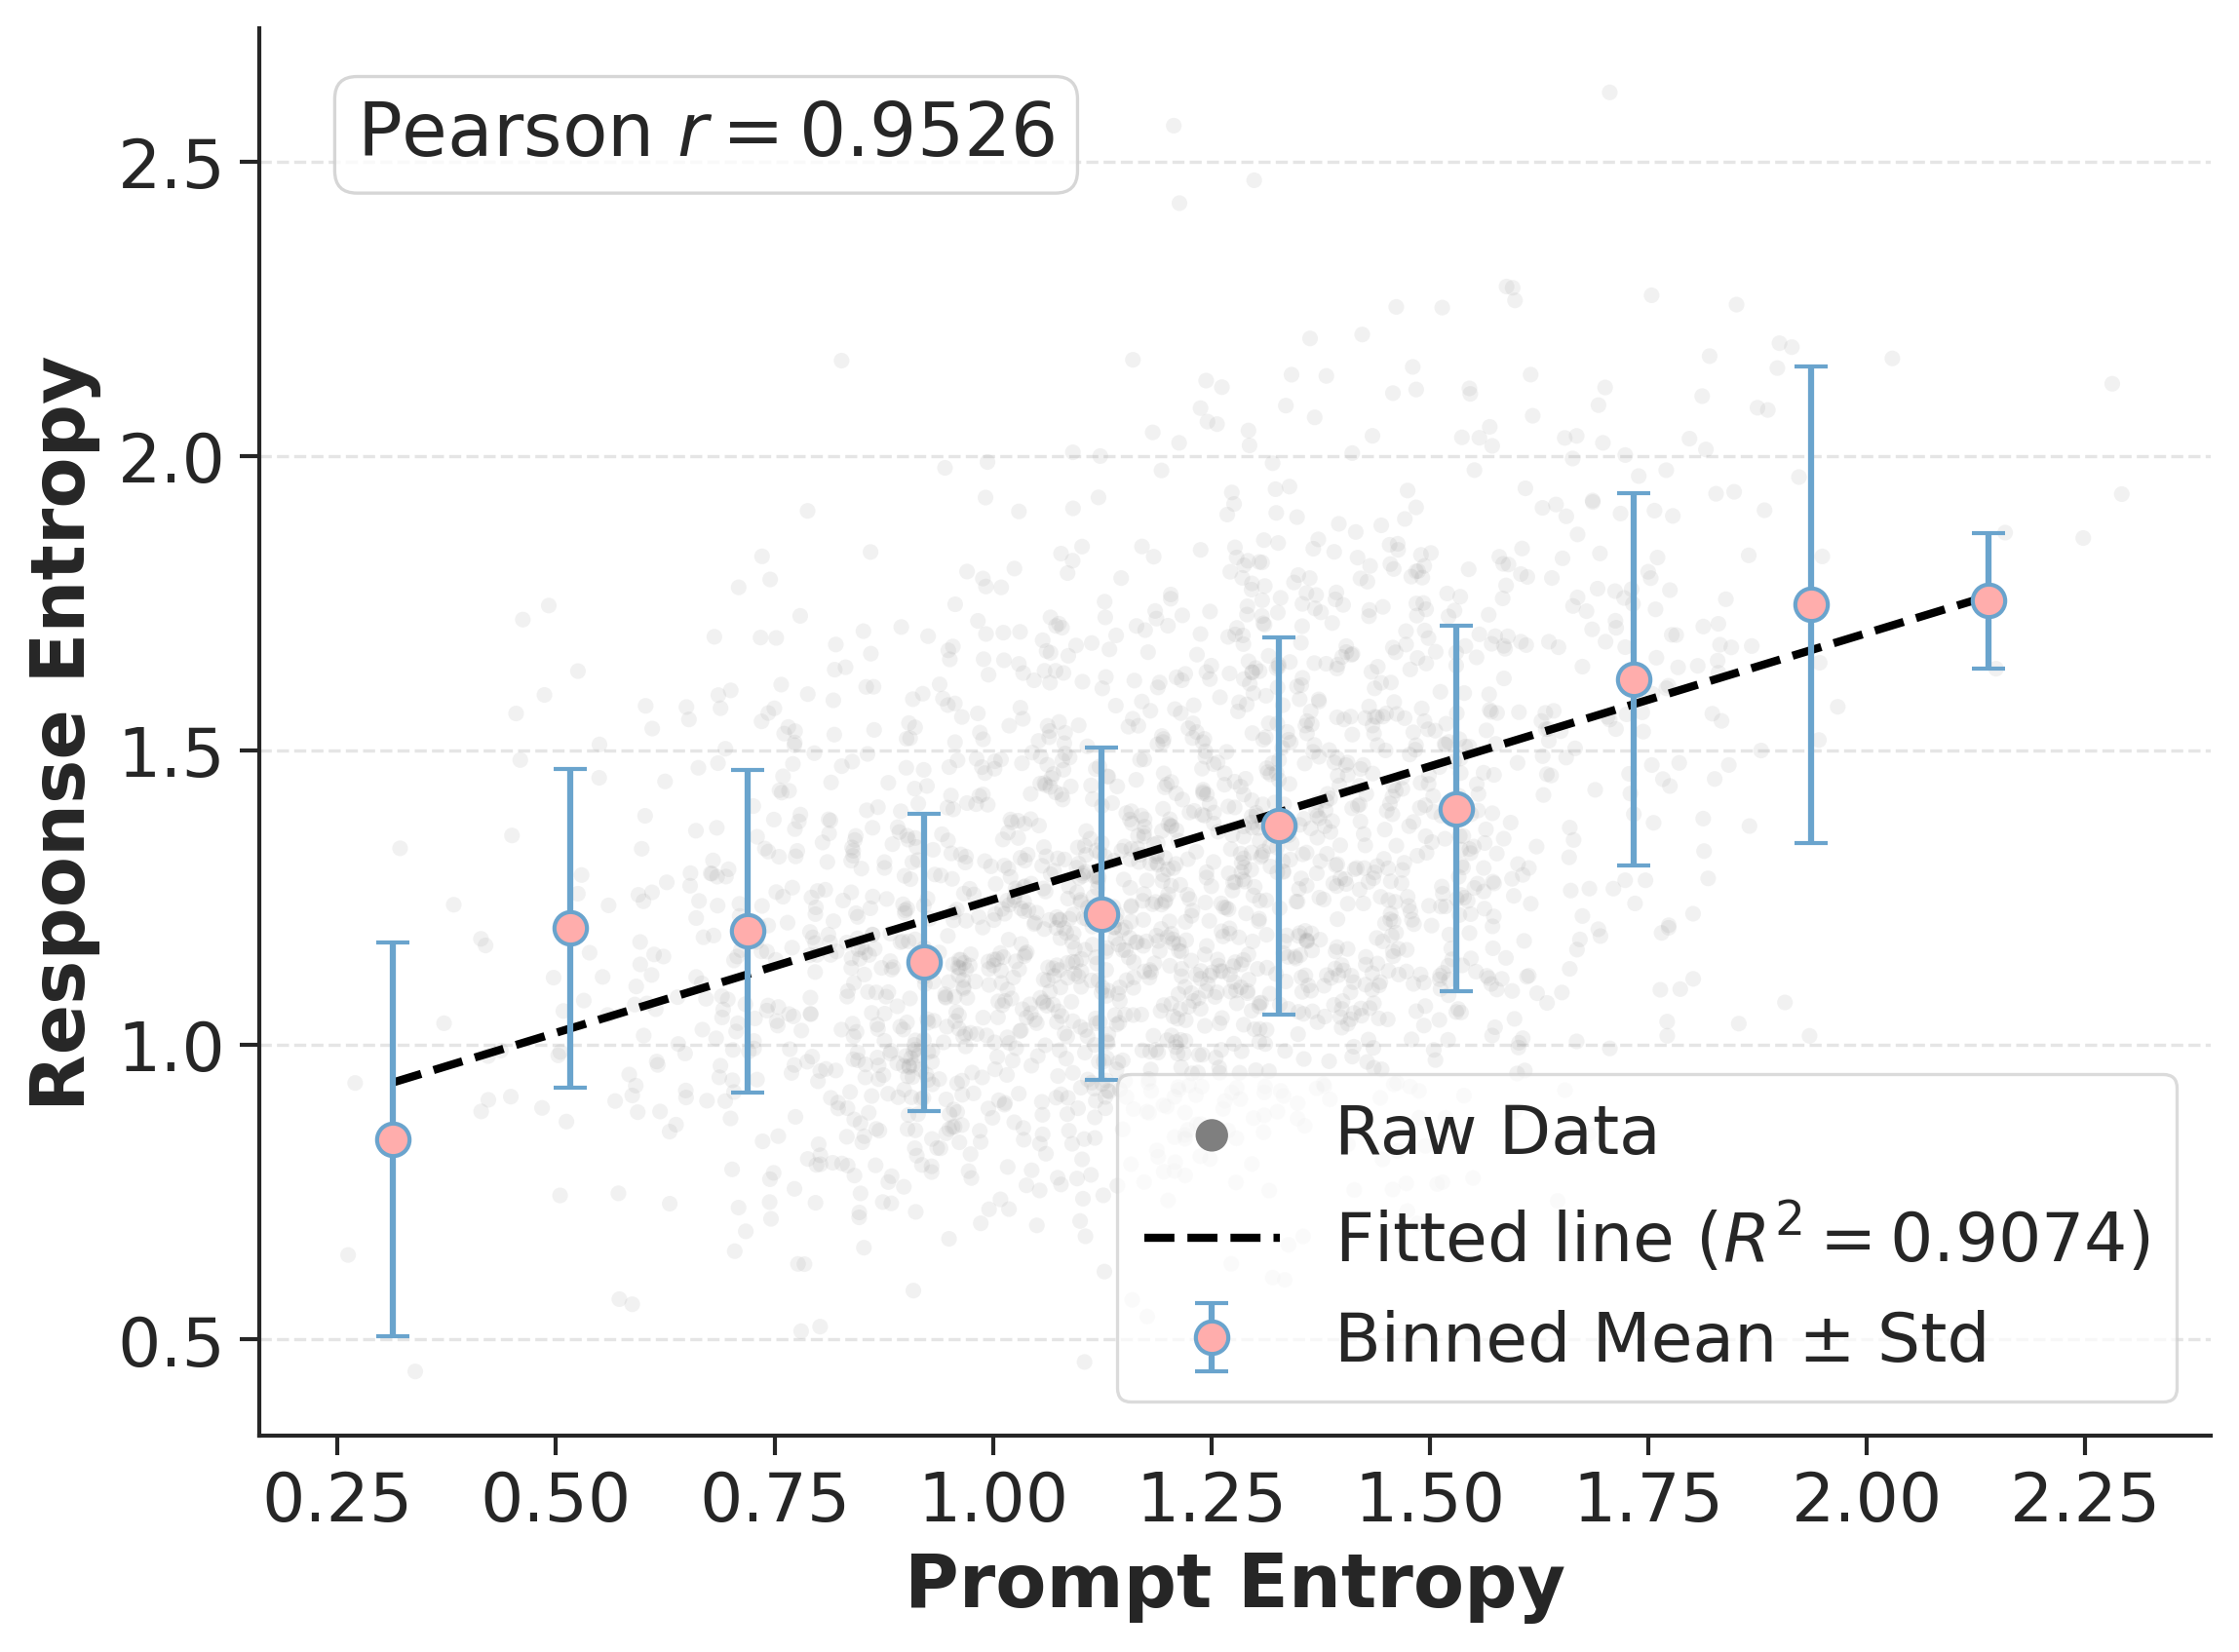
\includegraphics[width=\linewidth]{figures/appendix/binned_mean_respRatio10.png}
        \caption{$r=10\%$}
        \label{fig:respRatio10}
    \end{subfigure}
    \hfill
    \begin{subfigure}[b]{0.45\linewidth}
        \centering
        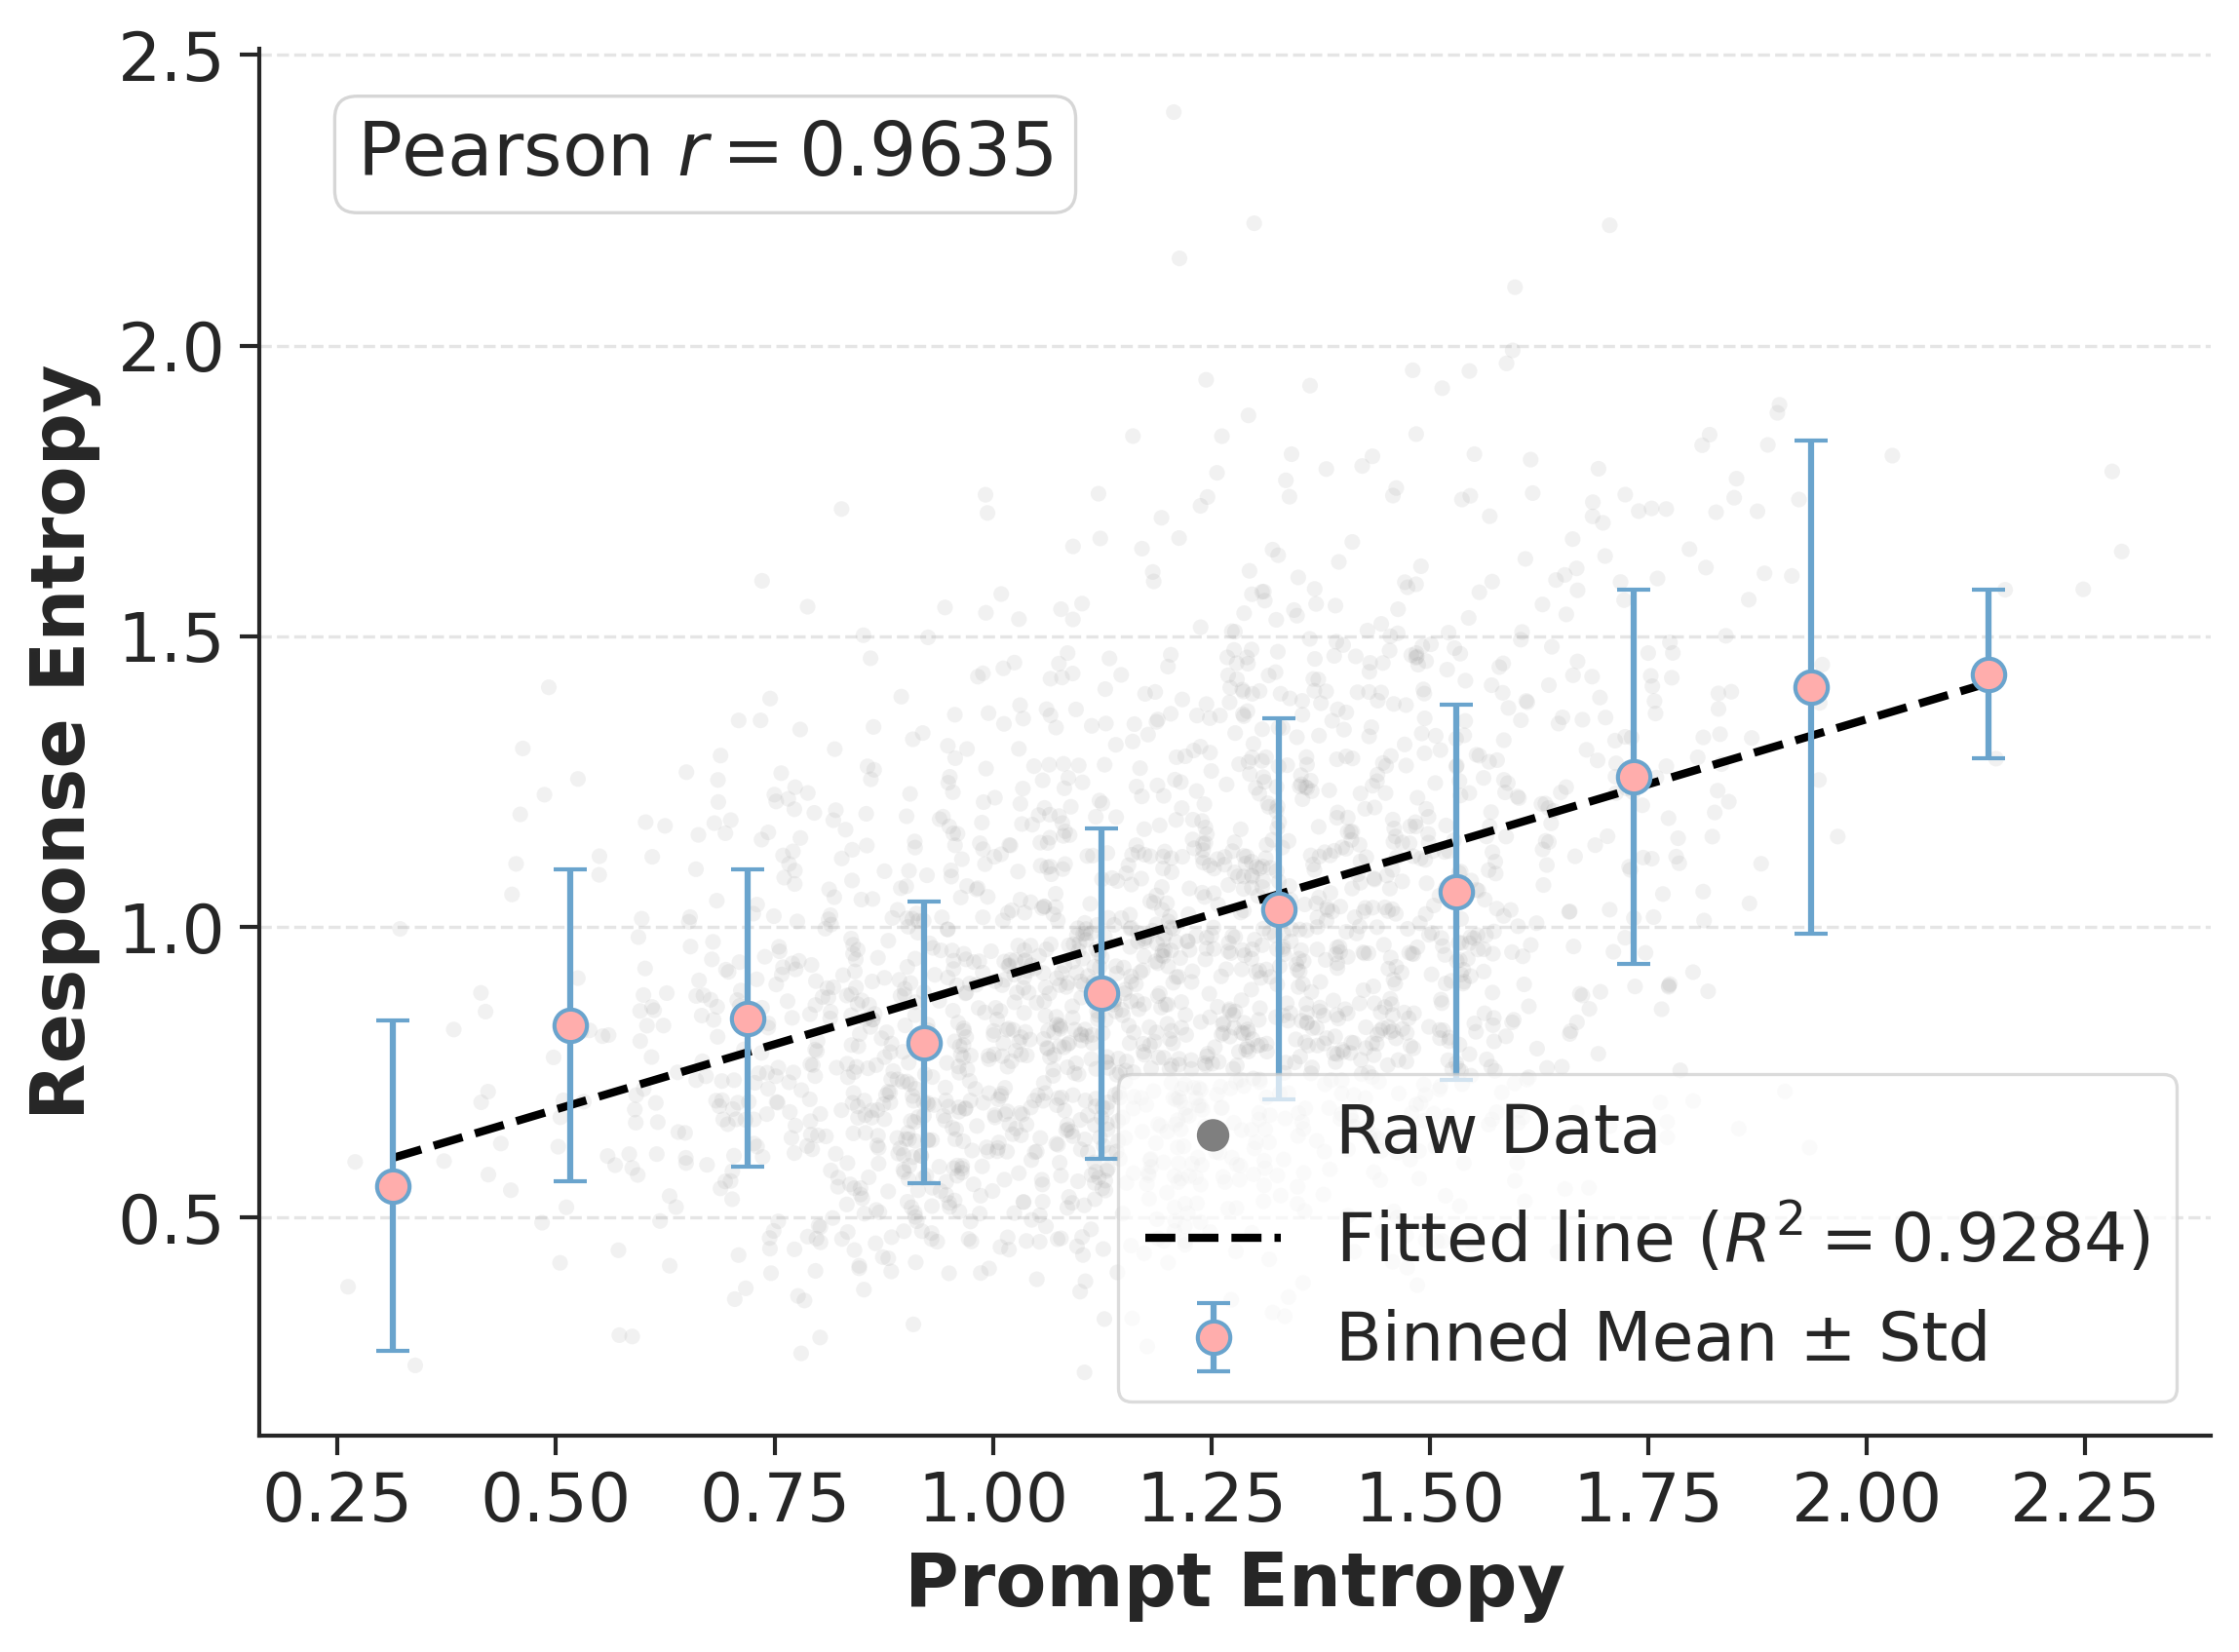
\includegraphics[width=\linewidth]{figures/appendix/binned_mean_respRatio20.png}
        \caption{$r=20\%$}
        \label{fig:respRatio20}
    \end{subfigure}

    \vspace{0.8em} % 行间距，可按版面微调

    % Row 2
    \begin{subfigure}[b]{0.45\linewidth}
        \centering
        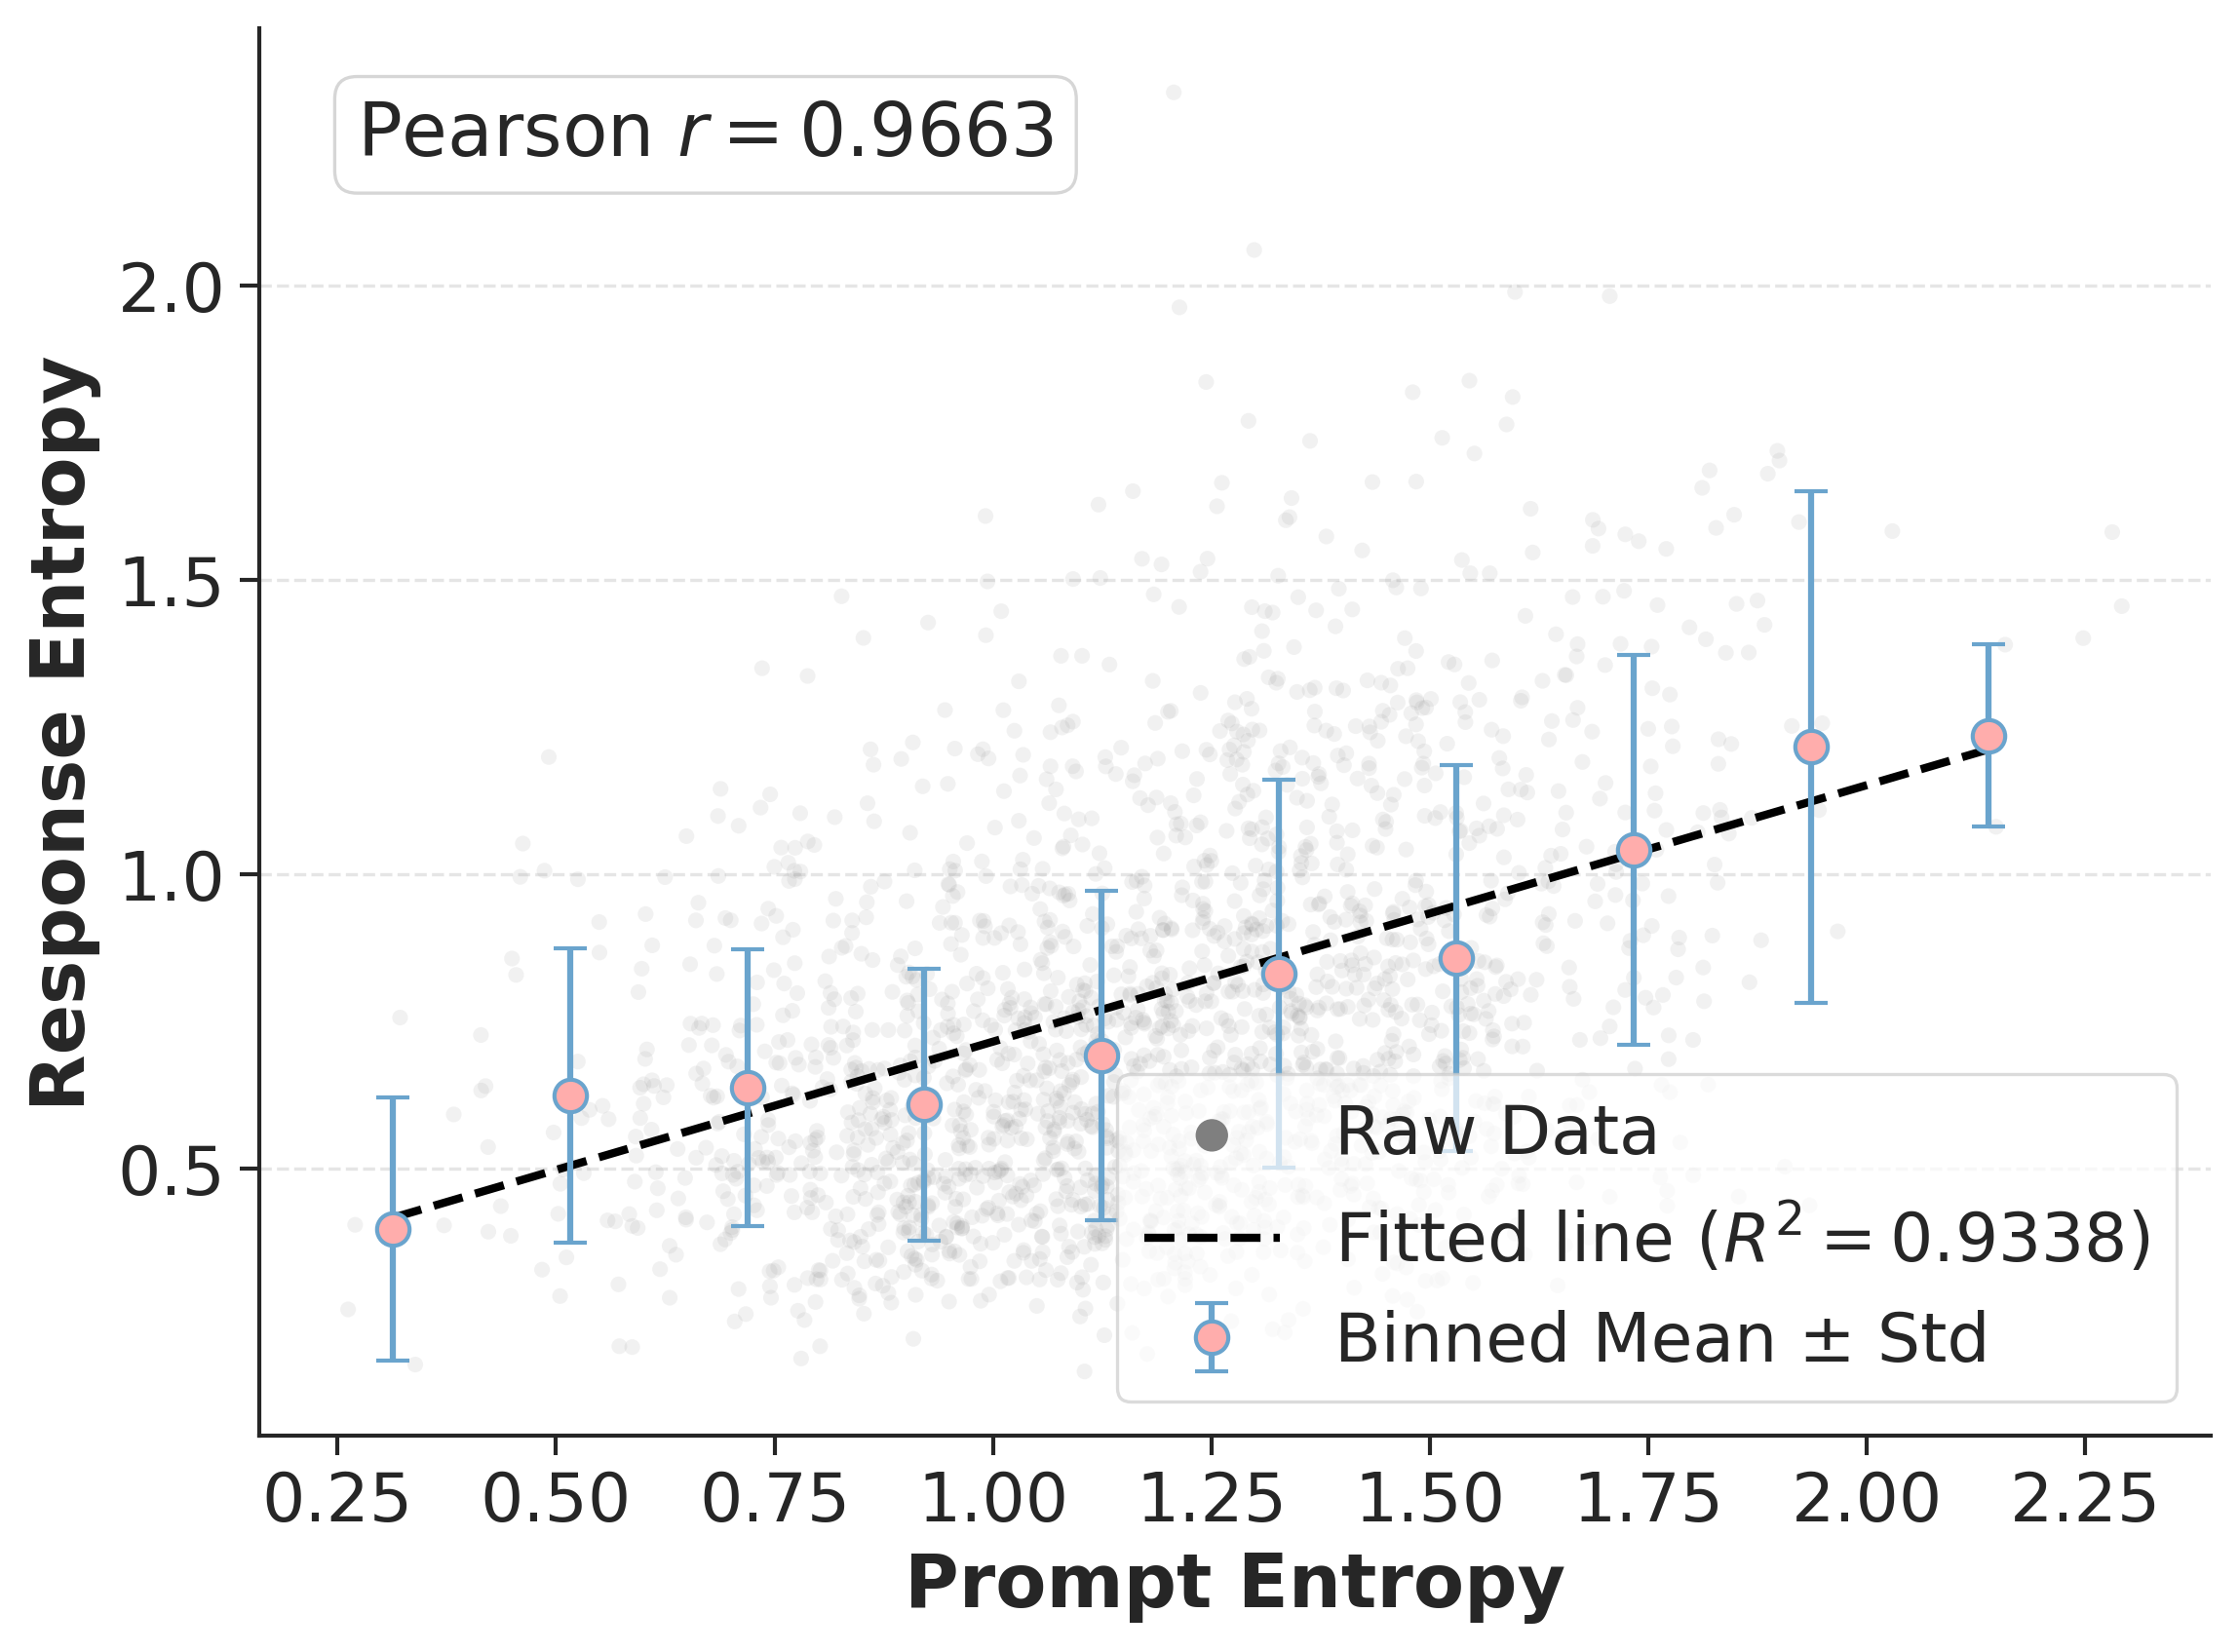
\includegraphics[width=\linewidth]{figures/appendix/binned_mean_respRatio30.png}
        \caption{$r=30\%$}
        \label{fig:respRatio30}
    \end{subfigure}
    \hfill
    \begin{subfigure}[b]{0.45\linewidth}
        \centering
        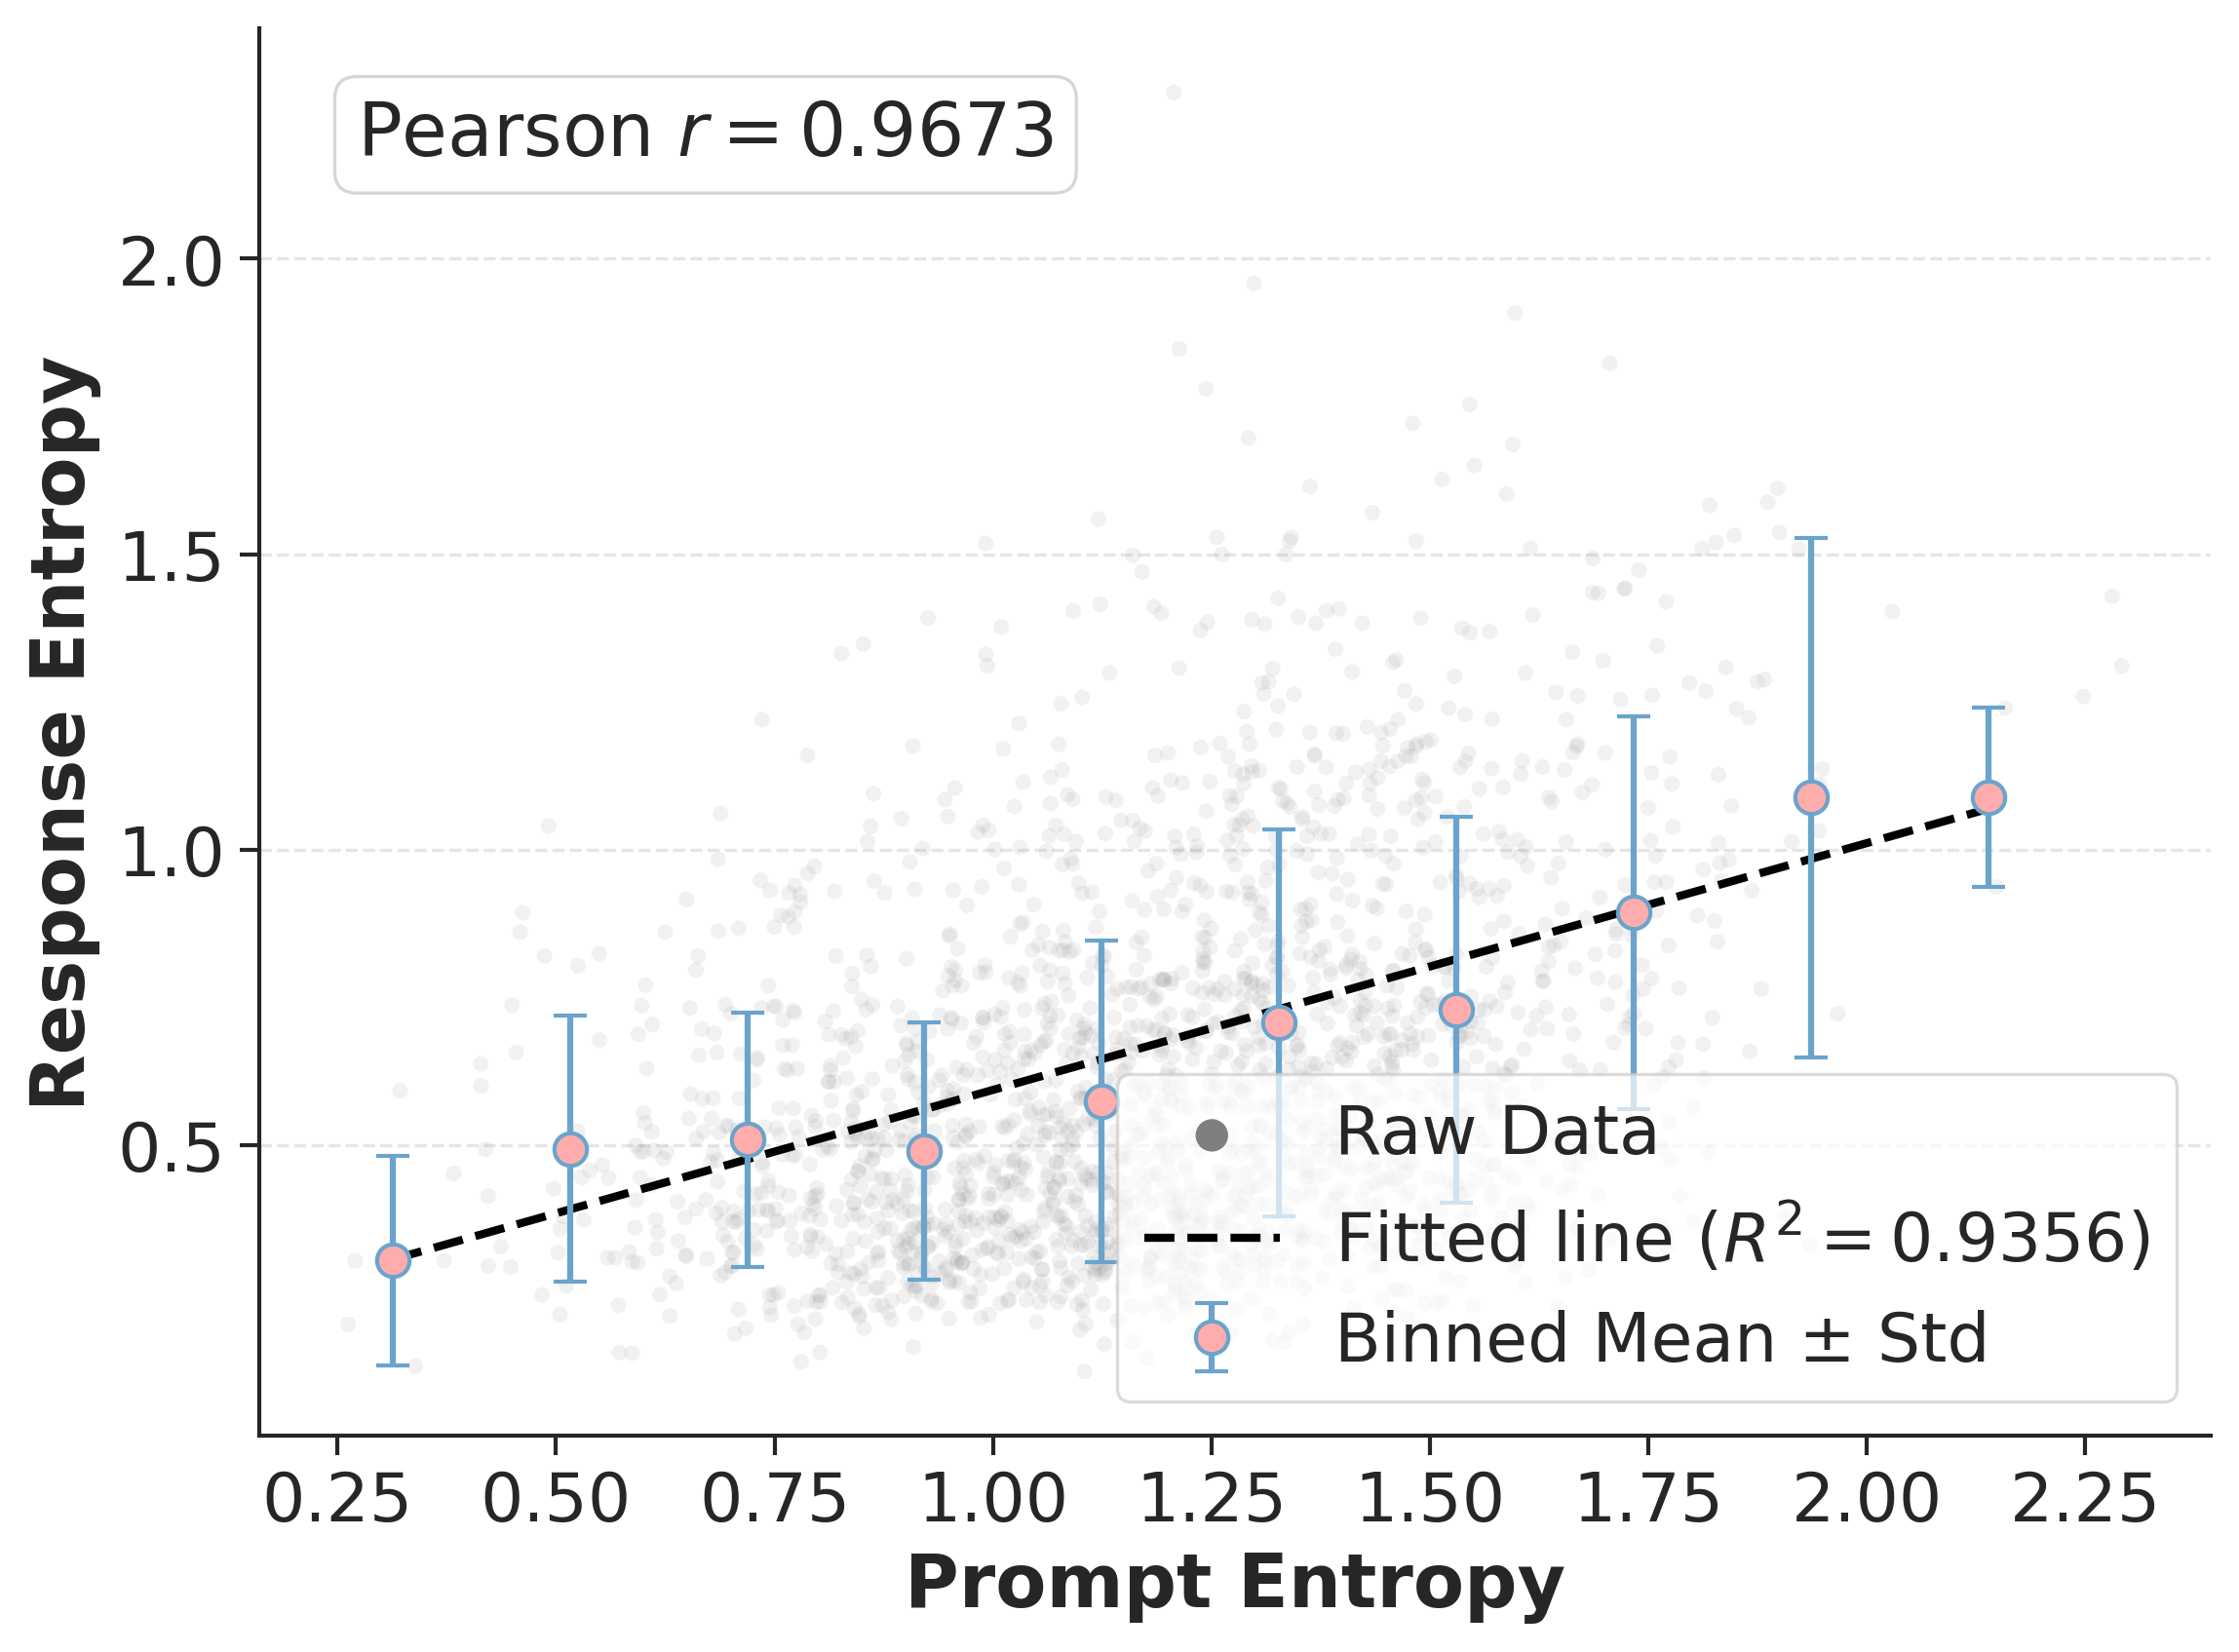
\includegraphics[width=\linewidth]{figures/appendix/binned_mean_respRatio40.png}
        \caption{$r=40\%$}
        \label{fig:respRatio40}
    \end{subfigure}
    
    \caption{Relationship between prompt entropy and response entropy computed over the top-$r\%$ tokens in the response distribution, sweeping $r\in\{10,20,30,40\}$. Each panel reports the binned mean trend under the corresponding ratio setting.}
    \label{fig:combined_results_appendix}
\end{figure}

\section{Additional Experiments}
\label{appendix-sec:additional-exp}
\subsection{Correlation Between Prompt Entropy and Response Entropy}

Building on the empirical validation of Assumption \ref{ass:propagation}, we conduct an additional robustness study by redefining the response entropy $S_{\mathrm{resp}}(x)$ as the entropy computed over only the top-$r\%$ tokens of the response distribution, sweeping $r \in \{10,20,30,40\}$. To suppress intrinsic decoding stochasticity, we follow the same binned-mean protocol on 2{,}048 prompts, binning by $S_{\mathrm{prompt}}(x)$ (proxied by $V(x)$) and averaging $S_{\mathrm{resp}}^{(r)}(x)$ within each bin. As shown in Figure~\ref{fig:combined_results_appendix}, the prompt--response relationship remains strongly linear across all ratios.
This indicates that the prompt--response entropy relationship is robust to this response-entropy definition, further supporting the bounded-noise linear approximation used in Assumption~\ref{ass:propagation}.
 





\subsection{Case Study}

To gain deeper insight into the behavior of our selective filtering algorithm, we analyze a case study based on prompts from the MATH dataset. 
We divide these prompts into four categories: Frequently Skipped Prompts (Easy), Frequently Skipped Prompts (Hard), Frequently Selected Prompts, and Prompts Frequently Selected by Stage 1 but Skipped by Stage 2.
We observe that frequently skipped easy prompts often involve simple computations or routine use of formulas, leading to high solution rates across sampled responses. In contrast, hard prompts that are often skipped tend to be too difficult for the model, leading to low or zero success across rollouts, limiting their value for training.
Frequently selected prompts tend to be moderately difficult, making consistent contributions to model learning. 
Furthermore, we analyze the prompts selected in stage 1 but filtered after stage 2. 
Most prompts are relatively easy, showing that the historical information is not reliable for filtering.



\begin{tcolorbox}[casestudy={Frequently Skipped Prompts (Easy)}]
1. \textbf{Question:} What is the value of $(2x + 5)^2$ when $x = 3$? \textbf{Solution:} 121.
\vspace{0.2cm}

2. \textbf{Question:} Solve for $x$: $5^{x + 4} = 125^x$?  
\textbf{Solution:} 21.
\vspace{0.2cm}

3. \textbf{Question:} A squirrel travels at a constant 4 miles per hour. How long does it take for this squirrel to travel 1 mile? Express your answer in minutes.  
\textbf{Solution:} 15.
\vspace{0.2cm}

4. \textbf{Question:} Evaluate $\text{log}_5 625$.  
\textbf{Solution:} 4.
\vspace{0.2cm}

5. \textbf{Question:} What value of $x$ will give the minimum value for $x^2- 10x + 24$? 
\textbf{Solution:} 5.
\end{tcolorbox}


\begin{tcolorbox}[casestudy={Frequently Skipped Prompts (Hard)}]
1. \textbf{Question:} Let $\triangle{PQR}$ be a right triangle with $PQ = 90$, $PR = 120$, and $QR = 150$. Let $C_{1}$ be the inscribed circle. Construct $\overline{ST}$ with $S$ on $\overline{PR}$ and $T$ on $\overline{QR}$, such that $\overline{ST}$ is perpendicular to $\overline{PR}$ and tangent to $C_{1}$. Construct $\overline{UV}$ with $U$ on $\overline{PQ}$ and $V$ on $\overline{QR}$ such that $\overline{UV}$ is perpendicular to $\overline{PQ}$ and tangent to $C_{1}$. Let $C_{2}$ be the inscribed circle of $\triangle{RST}$ and $C_{3}$ the inscribed circle of $\triangle{QUV}$. The distance between the centers of $C_{2}$ and $C_{3}$ can be written as $\sqrt {10n}$. What is $n$?
\textbf{Solution:} 725.
\vspace{0.2cm}

2. \textbf{Question:} Consider the region $A^{}_{}$ in the complex plane that consists of all points $z^{}_{}$ such that both $\frac{z^{}_{}}{40}$ and $\frac{40^{}_{}}{\overline{z}}$ have real and imaginary parts between $0^{}_{}$ and $1^{}_{}$, inclusive. Find the area of $A.$
\textbf{Solution:} $1200 - 200 \pi$.
\vspace{0.2cm}

3. \textbf{Question:} Ephram is growing $3$ different variants of radishes in a row of $13$ radishes total, but he forgot where he planted each radish variant and he can't tell what variant a radish is before he picks it. Ephram knows that he planted at least one of each radish variant, and all radishes of one variant will form a consecutive string, with all such possibilities having an equal chance of occurring. He wants to pick three radishes to bring to the farmers market, and wants them to all be of different variants. Given that he uses optimal strategy, the probability that he achieves this can be expressed as $\frac{m}{n}$, where $m$ and $n$ are relatively prime positive integers. Find $m+n$.  
\textbf{Solution:} 17.
\vspace{0.2cm}

4. \textbf{Question:} There are 1000 rooms in a row along a long corridor. Initially, the first room contains 1000 people, and the remaining rooms are empty. Each minute, the following happens: for each room containing more than one person, someone in that room decides it is too crowded and moves to the next room. All these movements are simultaneous (so nobody moves more than once within a minute). After one hour, how many different rooms will have people in them?  
\textbf{Solution:} 31.
\vspace{0.2cm}

5. \textbf{Question:} A regular hexagon has side length \(6\). Congruent arcs with radius \(3\) are drawn with the center at each of the vertices, creating circular sectors as shown. The region inside the hexagon but outside the sectors is shaded as shown. The original answer is in the form \(a\sqrt{b}-c\pi\). Please find the value of a + b + c.
\textbf{Solution:} 75.
\end{tcolorbox}


\begin{tcolorbox}[casestudy={Frequently Selected Prompts After Stage 2}]
1. \textbf{Question:} Let $z$ be a complex number such that
\[|z - 12| + |z - 5i| = 13.\]
Find the smallest possible value of $|z|.$ \textbf{Solution:} $\frac{60}{13}$.
\vspace{0.2cm}

2. \textbf{Question:} Find all real solutions to $x^4+(2-x)^4=34$.  Enter all the solutions, separated by commas.  
\textbf{Solution:} $1 + \sqrt{2}, 1 - \sqrt{2}$.
\vspace{0.2cm}

3. \textbf{Question:} Let b be a real number randomly selected from the interval $[-17,17]$. Then, m and n are two relatively prime positive integers such that m\/n is the probability that the equation $x^4+25b^2=(4b^2-10b)x^2$ has $\textit{at least}$ two distinct real solutions. Find the value of $m+n$. 
\textbf{Solution:} 63.
\vspace{0.2cm}

4. \textbf{Question:} Let $a,$ $b,$ $c,$ $d$ be real numbers such that\[\\frac{(a - b)(c - d)}{(b - c)(d - a)} = \\frac{2}{5}.\]Find the sum of all possible values of\[\frac{(a - c)(b - d)}{(a - b)(c - d)}.\]  
\textbf{Solution:} $-\frac{3}{2}$.
\vspace{0.2cm}

5. \textbf{Question:} The function $f$, defined on the set of ordered pairs of positive integers, satisfies the following properties: 
\begin{align*}  f(x,x) &=x, \\  f(x,y) &=f(y,x), \quad \text{and} \\ (x + y) f(x,y) &= yf(x,x + y).  
\end{align*}
Calculate $f(14,52)$. 
\textbf{Solution:} 364.
\end{tcolorbox}


\begin{tcolorbox}[casestudy={Prompts Frequently Selected by Stage 1 but Skipped by Stage 2}]
1. \textbf{Question:} A polynomial with integer coefficients is of the form
\[9x^4 + a_3 x^3 + a_2 x^2 + a_1 x + 15 = 0.\]
Find the number of different possible rational roots of this polynomial.
\textbf{Solution:} 16.
\vspace{0.2cm}

2. \textbf{Question:} When an integer is divided by 15, the remainder is 7. Find the sum of the remainders when the same integer is divided by 3 and by 5.  
\textbf{Solution:} 3.
\vspace{0.2cm}

3. \textbf{Question:} Find the number of positive divisors of 2002.  
\textbf{Solution:} 16.
\vspace{0.2cm}

4. \textbf{Question:} What is the base five product of the numbers $121_{5}$ and $11_{5}$?
\textbf{Solution:} 1331.
\vspace{0.2cm}

5. \textbf{Question:} If $\sin x = 3 \cos x,$ then what is $\sin x \cos x$ 
\textbf{Solution:} $\frac{3}{10}$.
\end{tcolorbox}
